\chapter{Eindontwerp}
In dit hoofdstuk wordt onderzocht hoe de bevindingen vanuit dit rapport geimplementeerd kunnen worden voor Jansje.\\

\section{Eisen}
Voor een praktische implementatie zijn de volgende eisen belangrijk:
\begin{enumerate}
    \item Ruimte is niet essentieel voor eigenaar
    \item Beschermt tegen regen
    \item Voldoet aan brandveiligheidseisen
    \item Bereikbaar voor onderhoud
    \item Minimale GM van >0.15 volgens IMO-eisen \cite{IMO_A749}
  
\end{enumerate}\\


De batterijen thermisch geisoleerd zijn van de warmtebronnen (moto/uitlaat).\\
Bereikbaar voor onderhoud; hiermee wordt bedoeld dat een monteur de ruimte in moet kunnen en de batterijkabels aan de voor- en achterkant goed moet kunnen zien of daar makkelijk voor moet kunnen zorgen.\\
Water bij een elektrisch systeem is ongewenst voor de veiligheid door kortsluiting en slijtage.\\
Lage GM betekent dat de batterijen niet te hoog moeten zijn om het schip instabiel te maken.
\section{Beschikbare ruimtes}
Het schip kan in vijf ruimtes opgedeeld worden hier beneden schematisch weergegeven, de rode lijnen in figuur \ref{fig:Bovenkant} zijn de loop paden, de blauwe strepen geven aan op welke pekken van het dek daadwerkelijk nuttige ruime is.
\begin{figure}
    \centering
    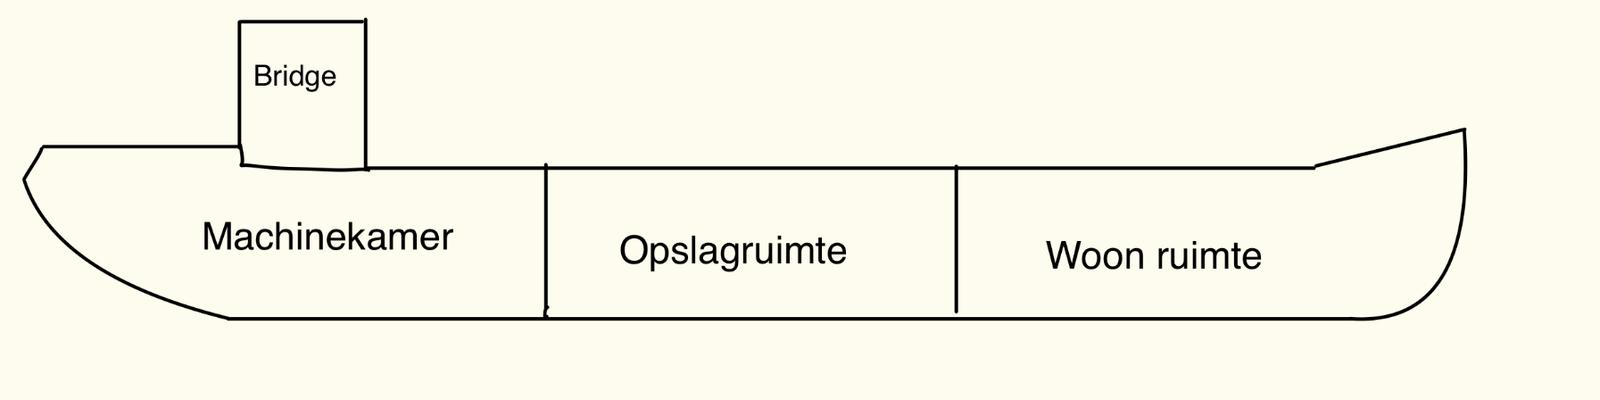
\includegraphics[width=0.8\linewidth]{vanaf de zijkant.jpeg}
    \caption{Zijprofiel van ruimtes}
    \label{fig:zijkant}
\end{figure}
\begin{figure}
    \centering
    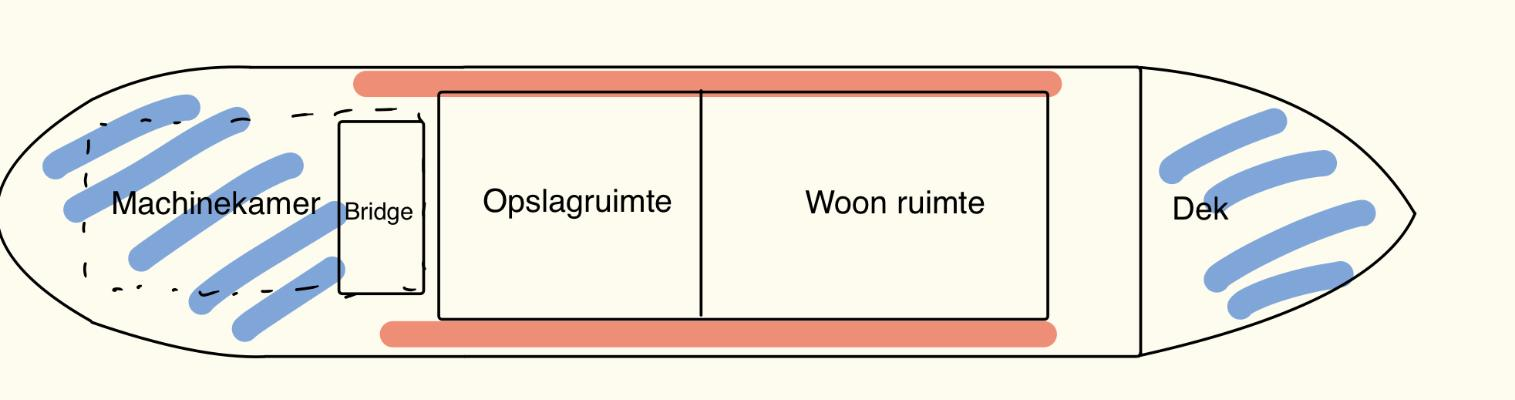
\includegraphics[width=0.8\linewidth]{vanaf boven.jpeg}
    \caption{Bovenprofiel van ruimtes}
    \label{fig:Bovenkant}
\end{figure}
\newpage
Nu worden de ruimtes getoetst aan de eerder gestelde eisen.\\
\\
De Bridge- en Woonruimte zijn essentieel voor de eigenaar en vallen af (eis 1).\\
Het dek is niet geschikt omdat deze niet tegen regen beschermt (eis 2).\\
Volgens ES-TRIN 2025 10.11 3 \cite{cesni2025inlandstandards} voldoet de machinekamer niet aan  brandveiligheidsseisen eis(3).\\
Alle ruimtes kunnen zo ingericht worden zodat ze bereikbaar zijn voor onderhoud (eis 4).\\
Omdat de bridge en het dek op het oppervlak van het schip zijn is de KG hoog (eis 5).\\
Dit wordt gevisualiseerd in de volgende matrix:

\begin{table}[htbp]
\centering
\caption{Evaluatie van scheepsruimtes op basis van functionele eisen}
\label{tab:ruimte_evaluatie}
\begin{tabular}{p{5cm}ccccc}
\toprule
\textbf{Functionele eis} & \textbf{Machinekamer} & \textbf{Opslagruimte} & \textbf{Woonruimte} & \textbf{Dek} & \textbf{Bridge} \\
\midrule
1. Ruimte is niet essentieel voor eigenaar & \cmark & \cmark & $\times$   & \cmark & $\times$   \\
\addlinespace
2. Beschermt tegen regen                   & \checkmark & \checkmark & \checkmark & $\times$   & \checkmark \\
\addlinespace
3. Voldoet aan brandveiligheidseisen       & $\times$   & \checkmark & \checkmark & \checkmark & \checkmark \\
\addlinespace
4. Bereikbaar voor onderhoud               & \checkmark & \checkmark & \checkmark & \checkmark & \checkmark \\
\addlinespace
5. Lage GM (Zwaartepunt)                   & \checkmark & \checkmark & \checkmark & $\times$   & $\times$   \\
\bottomrule
\end{tabular}
\end{table}
Dit geeft de volgende schematische weergave:
\begin{figure}[H]
    \centering
    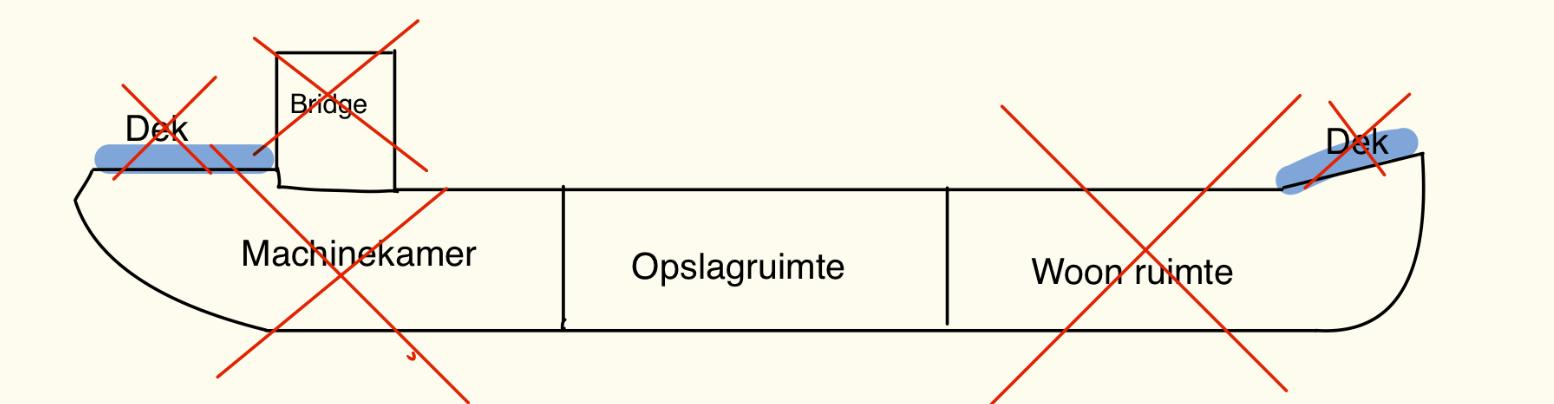
\includegraphics[width=0.8\linewidth]{afvallers.jpeg}
    \caption{Afvallers}
    \label{fig:Afvallers}
\end{figure}
Oftewel alleen de opslagruimte is als enige een optie voor de opslag van batterijen.
\newpage
\section{Inrichting opslagruimte}
Alhoewel alleen de opslagruimte een optie is, zijn er verschillende manieren om deze in te richten. Deze inrichtingen hebben invloed op eis 3, 4 en 5 en dus afgewogen om zo tot de beste inrichting te komen.\\
Voor eis 3 is er gekeken naar de richtlijnen die de Deense Maritieme Autoriteit heeft opgesteld, gevolgd. Deze worden gezien als de basis voor de toekomstige internationale regelgeving \cite{DMA_battery_operation_ships}.
\begin{itemize}
    \item De batterijruimte zal vrij zijn van hittebronnen en beschermd zijn tegen externe hitte door middel van hittebestendige isolatie.
    \item Er moet geschikt blusmateriaal aanwezig zijn voor een elektrische brand.
\end{itemize}\\

Voor eis 4 is er geen harde eis op een bepaalde afstand, het belangrijkst is dat de inspecteur/monteur door een bepaald looppad kan lopen om voor de batterij te komen de breedte van dit pad is ongeveer 0.6 meter \cite{Loopadbreedte}. Ook moet vanaf boven 0.2m speling zijn voor bedrading en dergelijken. Na gesprekken met dr. Ten wordt aangeraden dat de voorkant van de batterij bereikbaar is.\\
\\
Voor eis 5 wordt een minimale $GM$-waarde van $0{,}15$~m gehanteerd. Dit staat ook in het IMO-minimum voor dwarsscheepse stabiliteit \cite{IMO_A749}.
Zoals aangetoond in hoofdstuk~\ref{sec:stab_berekening} voldoen alle 
ontwerpen aan dit criterium.
\\


Voor het varen op nominaal vermogen is een vermogen nodig van 11 KW. De zeezoutbatterijen beter zijn op basis van de criteria ten opzichte van lithium batterijen. Om toch zoveel mogelijk gebruik te maken van zeezoutbatterijen is gewenst dat deze minimaal het nominale vermogen van 11KW kunnen leveren. Voor het optrekken van 22KW zouden dan LFP batterijen toegevoegd worden. Om dit te realiseren hebben is er een serie aandrijving nodig zoals weergegeven in figuur \ref{fig:Aandrijving}, hierbij kan de zeezout batterij eventueel bij bijvoorbeeld het afremmen de LFP batterijen op te laden om deze in de gewenste batterijpercentage window te houden.
\\
\begin{figure}[H]
    \centering
    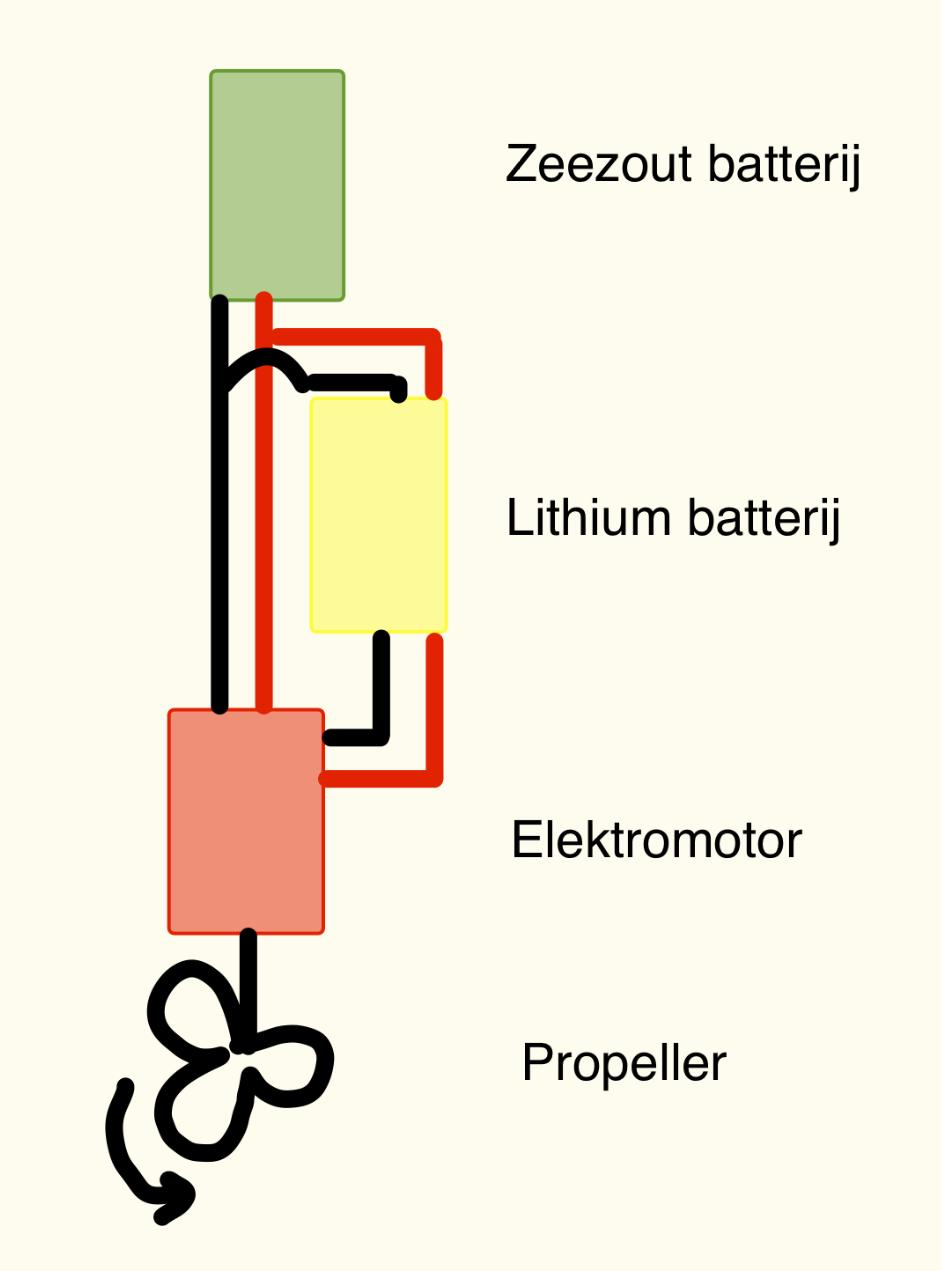
\includegraphics[width=0.5\linewidth]{aandrijving.jpeg}
    \caption{Serie aandrijving}
    \label{fig:Aandrijving}
\end{figure}
\\
\newpage
\paragraph{Zeezout}
\begin{equation*}
n_z = \left\lceil \frac{P_{\min,z}}{P_z} \right\rceil_5
    = \left\lceil \frac{10{,}8}{0{,}187} \right\rceil_5
    = \lceil 57{,}75 \rceil_5 = 60,
\qquad
E_z^{\text{lev}} = 60 \times 0{,}48 = 28{,}80\ \text{kWh}.
\end{equation*}

\paragraph{LFP (80\% operating window).}
\begin{equation*}
E_l^{\text{bruik}} = 0{,}80 \times 5{,}8 = 4{,}64\ \text{kWh},
\qquad
n_l = \left\lceil \frac{11{,}7}{5{,}9} \right\rceil_5 = \lceil 1{,}98 \rceil_5 = 5,
\qquad
E_l^{\text{lev}} = 5 \times 4{,}64 = 23{,}20\ \text{kWh}.
\end{equation*}

\paragraph{Capacity gap.}
\begin{equation*}
\Delta E = E_{\text{nodig}} - \bigl(E_z^{\text{lev}} + E_l^{\text{lev}}\bigr)
         = 108{,}15 - (28{,}80 + 23{,}20)
         = \boxed{56{,}15\ \text{kWh}}.
\end{equation*}

\\
Uit de berekening blijkt dat er ongeveer 60 zeezoutbatterijen toegevoegd moeten worden en ongeveer 5 LFP batterijen . De capaciteit van deze twee bij elkaar is totaal 52 kWh; er is totaal 108,15 kWh nodig, wat een capaciteitstekort van 56,15 KWh geeft. Deze kun je opvullen op verschillende manieren die verder worden uitgelicht in de ontwerpen.
\\
De ruimte is totaal 2.5x3x2 meter, oftewel 12 kubieke meter beschikbaar, waarbij lithiumbatterijen een hogere dichtheid hebben dan zeezoutbatterijen.
\\

Met het bovenstaande in gedachte kunnen drie ontwerpen afgewogen worden tegen elkaar.

\subsection{Ontwerp 1; zo duurzaam mogelijk }
Voor ontwerp 1 worden zoveel mogelijk zeezoutbatterijen toegevoegd en zo min mogelijk lithiumbatterijen.  De zeezoutbatterijen kunnen maximaal zeven hoog gestapelt worden en de LFP maximaal zes hoog, om te voldoen aan de voorwaardes en 2 meter hoog.

\begin{figure}[H]
    \centering
    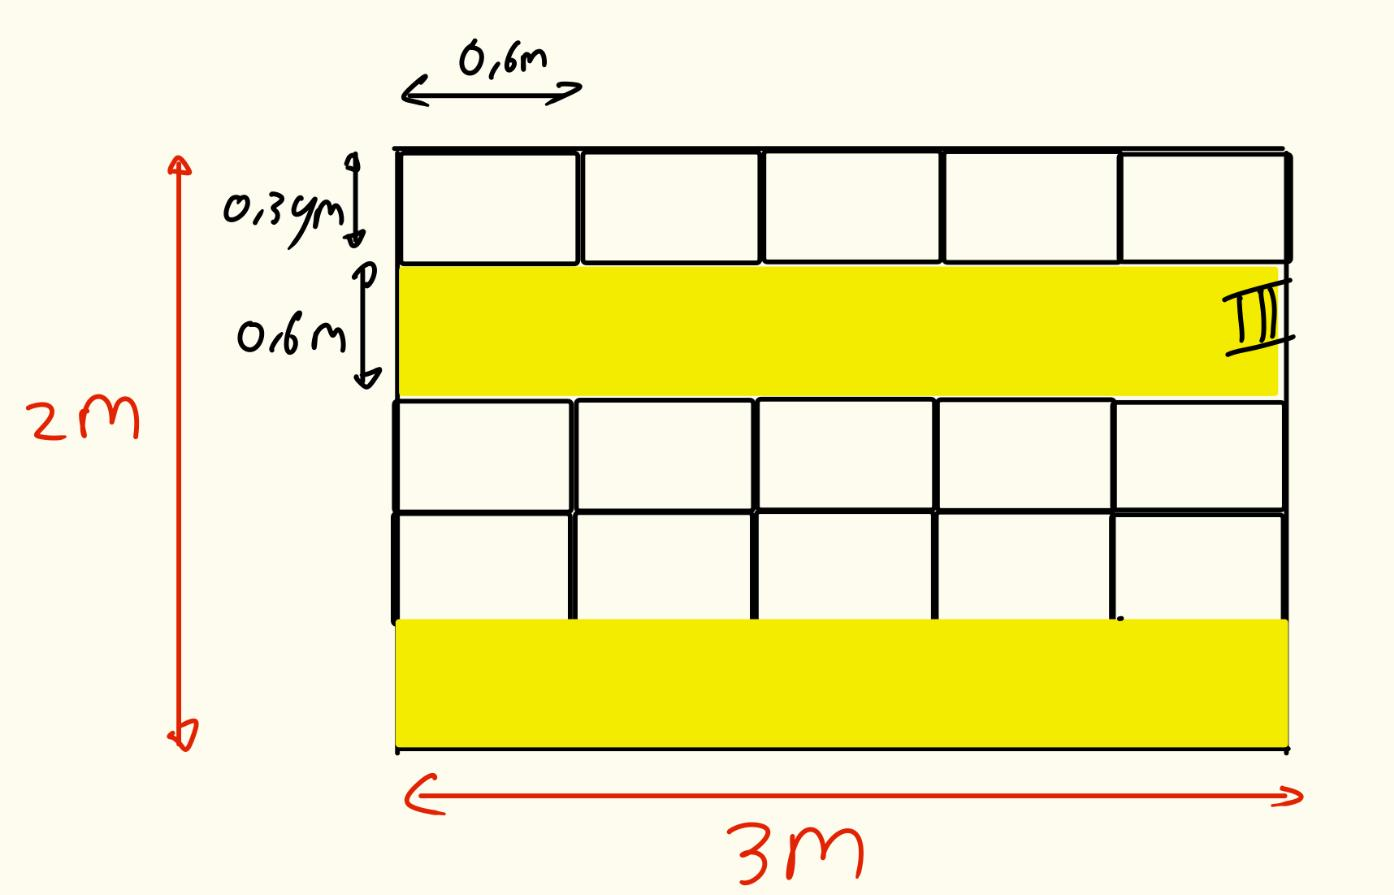
\includegraphics[width=0.5\linewidth]{inrichting alleen zeezout.jpeg}
    \caption{Initieele inrichting 1}
    \label{fig:Ontwerp 1}
\end{figure}\\

Op het figuur \ref{fig:Ontwerp 1} zijn 15 stapels mogelijk ofwel 105 batterijen. berekening, 50.4 KWh en 19.6 KW.
Elke stapel van zeezoutbatterijen die wordt vervangen door lithium voegt 29.12 KWh toe en 29.68 KW. Oftewel er moeten twee volle stapels van zeezout uit en twee volle stapels van lithium in om te voldoen aan de capiciteit van 108.15 KWh.
\begin{figure}[H]
    \centering
    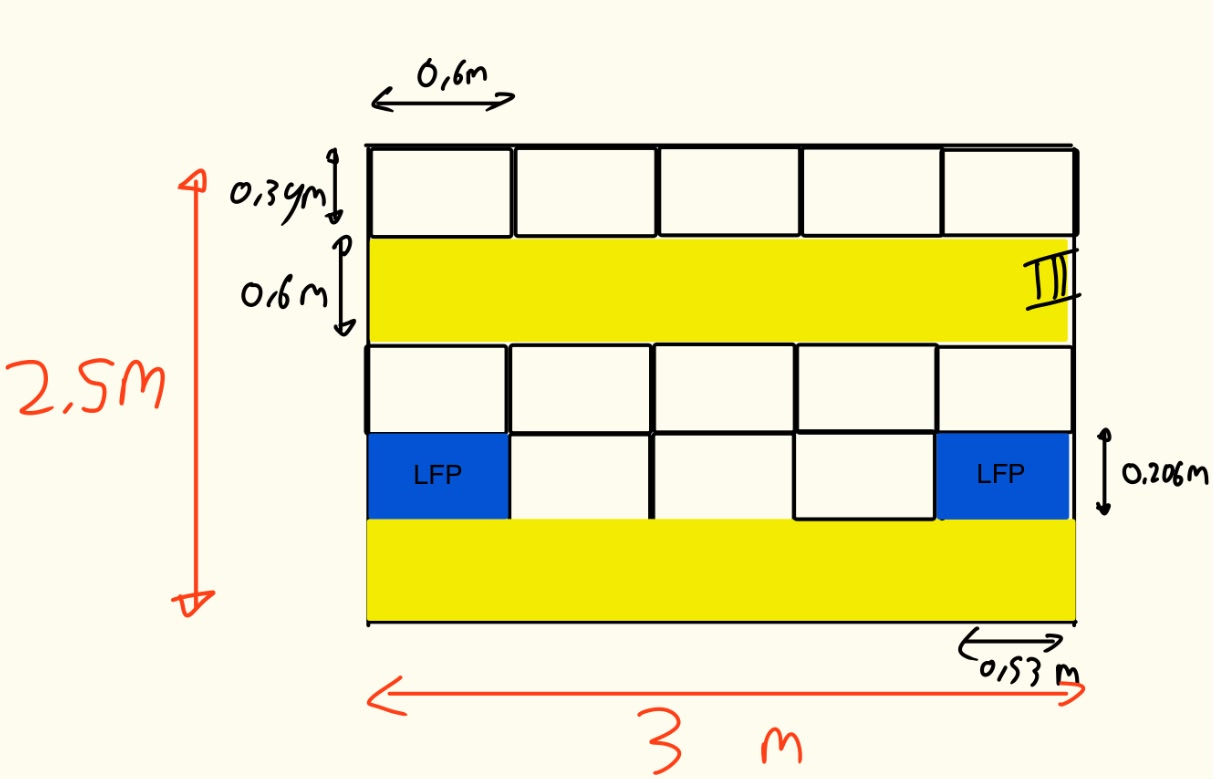
\includegraphics[width=0.5\linewidth]{setup A.jpeg}
    \caption{Ontwerp 1, blauw lithium, wit zeezout}
    \label{fig:Ontwerp 1}
\end{figure}\\
Bill of materials:\\
90 zeezoutbatterijen 88\%
12 LFP 12\%
102 totaal 100\%
\subsection{Ontwerp 2; zo goedkoop mogelijk}
Voor ontwerp 2 is het belangrijk dat de zeezoutbatterijen het nominale vermogen nog kunnen leveren, de rest wordt opgevangen door de LFP batterijen. Zoals eerder berekend \ref{} moeten er 60 zeezoutbatterijen en 18 lithiumbatterijen komen. Er is ruimte voor 16 stapels, de lithium batterij is het zwaarst dus die moet zo laag mogelijk zijn. Lithium worden 5 stapels totaal waarvan 3, 4 batterijen hoog zijn en de andere 2 stapels 3 batterijen hoog. Dan worden zeezoutbatterijen over 10 stapels allemaal van 6 hoog.
\begin{figure}[H]
    \centering
    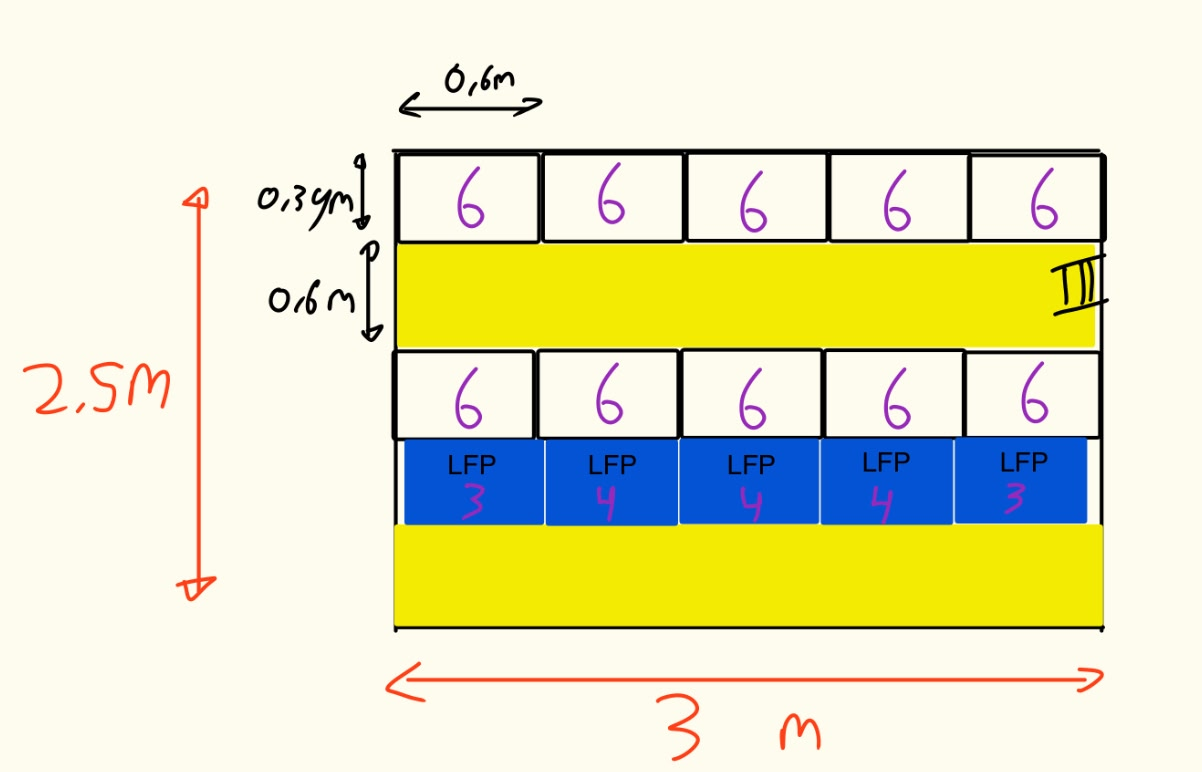
\includegraphics[width=0.6\linewidth]{design B.jpeg}
    \caption{Ontwerp 2, blauw lithium, wit zeezout}
    \label{fig:Ontwerp 1}
\end{figure}\\

Bill of materials:\\
90 zeezoutbatterijen 88\%
12 LFP 12\%
102 totaal 100\%
\subsection{Ontwerp 3; hybride van ontwerp 1 en ontwerp 2}
In ontwerp 1 en 2 is te zien dat er 15 stapels te maken zijn, waarvan tenminste 10 zeezout en 2 LFP moeten zijn. De overige 3 stapels kan zelf een combinatie voor gekozen worden, dat is design 3. Dit om een hybride combinatie tussen ontwerp 1 en 2 ook door te kunnen rekenen in de onderstaande gewogen criteria tabel.
\begin{figure}[H]
    \centering
    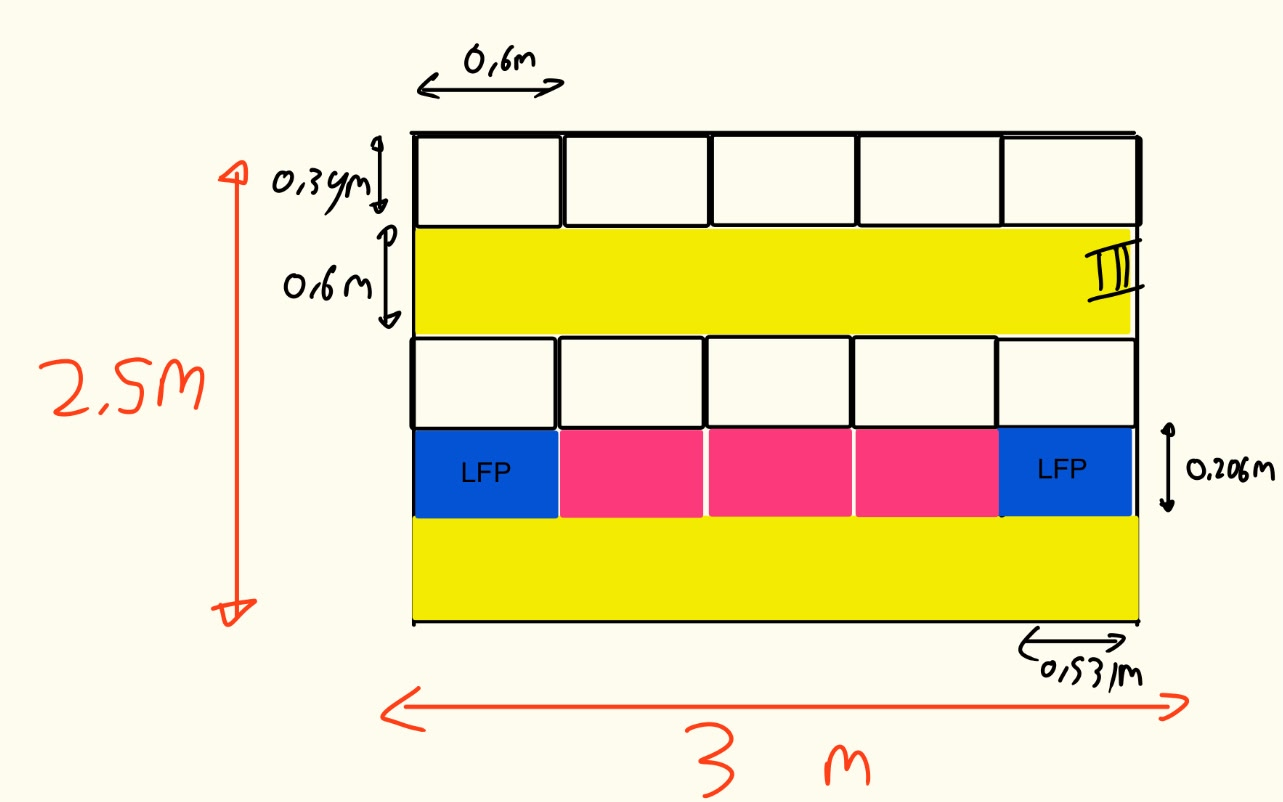
\includegraphics[width=0.6\linewidth]{Design C.jpeg}
    \caption{Ontwerp 3, waarbij roze zeezout of lfp kan zijn}
    \label{fig:Ontwerp 3}
\end{figure}\\

\subsection{Gewogen criteria tabel}
De designs worden afgewogen tegen elkaar, een groot deel van deze criteria  komen uit de gewogen criteria tabel van energieopslag [\ref{tab:allesheetdit}].\\
Omdat alle designs nominaal op zeezoutbatterijen kunnen varen, is de innovativiteit overal gelijk.

\begin{table}[H]
\centering
\caption{Scoretabel van energieopslagmethoden specifiek voor Jansje (genormaliseerde bronscores)}
\resizebox{\textwidth}{!}{
\begin{tabular}{lcccc}
\toprule
Criterium & Weging (\%) & Ontwerp 1 & Ontwerp 2 & Ontwerp 3\\
\midrule
Duurzaamheid                       & 16 & 4.87 & 4.76 & x \\
Innovativiteit                     & 15 & 4.74 & 4.50 & x \\
Kosten per effectieve kWh (€/kWh)  & 13 & 4.98 & 4.95 & x \\
Veiligheid                         & 13 & 4.87 & 4.75 & x \\
Levensduur (jaren)                 & 13 & 4.64 & 4.31 & x \\
CAPEX (€)                          & 12 & 1.50 & 1.94 & x \\
Efficiëntie (\%)                   & 10 & 4.99 & 4.98 & x \\
Massa (kg)                         &  8 & 1.63 & 2.10 & x \\
Totaal                             & 100 & 4.17 & 4.09 & x \\
\bottomrule
\end{tabular}
}
\label{tab:inrichting}
\end{table}

De scores zijn gebasseerd op de scores uit de gewogencriteria tabel voor energieopslag [\ref{tab:allesheetdit}], hierbij is gekeken naar de score van de batterij en het percentage van hoeveel deze voorkomt.\\
Bijvoorbeeld voor ontwerp 1: 88 procent van de batterijen is zeezoutbatterijen, de score in de tabel is 5.0 dus 0.88 x 5 = 4.4, LFP scoorde 3.94 dus 0.12 x 3.94 = 0.47, de totale score voor duurzaamheid wordt dan 4.87.
\begin{table}[h]
\centering
\caption{Scoretabel van energieopslagmethoden specifiek voor Jansje}
\resizebox{\textwidth}{!}{
\begin{tabular}{lcccccc}
\toprule
Criterium & Weging (\%) & LFP & Zeezoutbatterij (gen 4.0)\\
\midrule
Duurzaamheid                      & 16  & 3.94 & 5.00 \\
Innovativiteit                    & 15  & 2.83 & 5.00 \\
Kosten per effectieve kWh (€/kWh) & 13  & 4.80 & 5.00 \\
Veiligheid                        & 13  & 3.95 & 5.00 \\
Levensduur (jaren)                & 13  & 2.00 & 5.00 \\
CAPEX (€)                         & 12  & 5.00 & 1.02 \\
Efficiëntie (\%)                  & 10  & 4.90 & 5.00 \\
Massa (kg)                        &  8  & 5.00 & 1.19 \\
Totaal                            & 100 & 3.94 & 4.22 \\
\bottomrule
\end{tabular}
}
\label{tab:allesheetdit}
\end{table}

\section{CAD}
\begin{figure}[H]
    \centering
    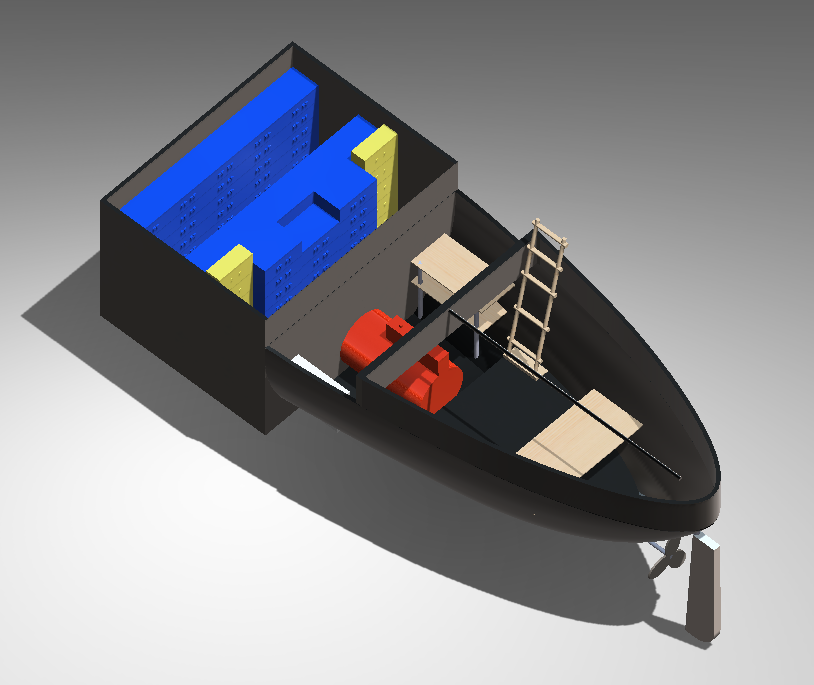
\includegraphics[width=0.9\linewidth]{Hoofdstukken/CAD.png}
    \caption{Ontwerp 1, blauw lithium, wit zeezout}
    \label{fig:Ontwerp 1}
\end{figure}\\